\documentclass[a4paper,12pt]{article}
\usepackage[utf8]{inputenc}
\usepackage[spanish]{babel}
\usepackage{tikz}
\usepackage{geometry}
\usepackage{setspace}
\usepackage{titlesec}
%\usepackage{lmodern}
\usepackage{multicol}
\usepackage{fancyhdr}
\usepackage{graphicx}
%\usepackage{helvet}
%\usepackage{mathptmx}
\usepackage{amsmath}       
\usepackage{amssymb}      
\usepackage{adjustbox}     
\usepackage{lastpage}
\usepackage{pgfplots}
\pgfplotsset{compat=1.17}
\usepackage{amsmath}
\usepackage{minted}
\usepackage{wrapfig}

\usepackage{tabularx}
\usepackage{qrcode}
\usepackage{tikz}
\usetikzlibrary{matrix, fit, positioning}

\usepackage{hyperref}
\usepackage{booktabs}
\usepackage{array}
\usepackage{float}
\usepackage{longtable}  

\renewcommand{\arraystretch}{1.4}
\setlength{\tabcolsep}{8pt} 

\setlength{\footskip}{25pt}
%---------------------------python
\usepackage[T1]{fontenc}
\usepackage[utf8]{inputenc}

\usepackage{listings}
\usepackage{xcolor}

\lstdefinestyle{pythonstyle}{
	language=Python,
	basicstyle=\ttfamily\small,
	keywordstyle=\color{blue},
	stringstyle=\color{red},
	commentstyle=\color{gray},
	numbers=left,
	numberstyle=\tiny\color{gray},
	stepnumber=1,
	numbersep=5pt,
	showspaces=false,
	showstringspaces=false,
	breaklines=true,
	frame=single,
	tabsize=4
}



%-------------------------------Consola
\usepackage{listings}
\usepackage{xcolor}

\lstdefinestyle{consola}{
	backgroundcolor=\color{black!5},
	basicstyle=\ttfamily,
	frame=single,
	keywordstyle=\color{blue},
	commentstyle=\color{gray},
	showstringspaces=false
}

%Plano Z y Z^2

\usepackage[utf8]{inputenc}
\usepackage{amsmath, amssymb}
\usepackage{pgfplots}
\pgfplotsset{compat=1.18}
\usepackage{geometry}
\geometry{a4paper, margin=2.5cm}


\geometry{top=2.5cm, bottom=2.5cm, left=2.5cm, right=1.5cm}

% Estilo de página
\pagestyle{fancy}
\fancypagestyle{miestilo}{
	\fancyhf{} % Limpia encabezado y pie
	
	% Encabezado izquierda: logo
	\fancyhead[L]{%
		\vspace{0.1cm}
		\adjustbox{valign=c,scale=0.15}{%
			\begin{tikzpicture}
				\clip (-3,-2.8) rectangle (3,2.8);
				\draw[black,line width=0.8cm] (-2.3,0)--(2.3,0);
				\draw[black,line width=0.8cm] (0,-2.85)--(0,2.85);
				\draw[black,line width=0.87cm] (0,2.8) circle(2);
				\draw[black,line width=0.87cm] (0,-2.8) circle(2);
			\end{tikzpicture}
		}%
	}
	
	% Encabezado centro: título
	\fancyhead[C]{\textbf{Técnicas Digitales 1   
	}}
	
	% Encabezado derecha: TP y año debajo
	\fancyhead[R]{%
		Guia Practica N°1 \\ 2026
	}
	
	% Línea en el encabezado y pie
	\renewcommand{\headrulewidth}{0.4pt}
	\renewcommand{\footrulewidth}{0.4pt}
	
	% Pie de página derecha: Página X de Y
	\fancyfoot[R]{Página \thepage\ de \pageref{LastPage}}
}


\begin{document}
	
	% --------- PORTADA ---------
	\pagestyle{empty}
	\begin{center}
		\textbf{\LARGE UNIVERSIDAD TECNOLÓGICA NACIONAL}\\[0.2cm]
		\textbf{\Large FACULTAD REGIONAL CÓRDOBA}\\[0.5cm]
		\textbf{\large INGENIERÍA ELECTRÓNICA}\\[1.5cm]
		
		\begin{tikzpicture}
			\clip (-3,-2.8) rectangle (3,2.8);
			\draw[black,line width=0.8cm] (-2.3,0)--(2.3,0);
			\draw[black,line width=0.8cm] (0,-2.85)--(0,2.85);
			\draw[black,line width=0.87cm] (0,2.8) circle(2);
			\draw[black,line width=0.87cm] (0,-2.8) circle(2);
		\end{tikzpicture}
		
		\vspace{1cm}
		\textbf{\huge Técnicas Digitales 1   
		}\\[0.5cm]
		\rule{\textwidth}{0.4pt}\\[0.3cm]
		\textbf{\Huge Guia Practica N°1
		}\\[0.3cm]
		{\large Introduccion a Verilog}\\[0.3cm]
		\rule{\textwidth}{0.4pt}\\[1.5cm]
	\end{center}
	
	\begin{flushleft}
		\begin{tabular}{@{}ll}
			DOCENTES     & : Esp.Ing. Marcelo Casasnovas\\ 
			& \ \  Ing Florencia Belén Molla JTP \\[0.2cm]
			CÁTEDRA      & :  Técnicas Digitales 1   \\[0.2cm]
			CURSO        & : 3R4 \\[0.2cm]
			ALUMNO      & :
			\begin{tabular}[t]{@{}l l}
				Gonza Elías Noel Imanol           & 87669 \\ 
			\end{tabular}
		\end{tabular}
	\end{flushleft}
	
	\vfill
	\begin{center}
		\textbf{CÓRDOBA, ARGENTINA}\\
		\textbf{2026}
	\end{center}
	\pagestyle{empty}
	% --------- CAMBIO DE ESTILO ---------
	\newpage
	\pagenumbering{arabic}
	\pagestyle{miestilo}
	% --------- CONTENIDO ---------
	\tableofcontents
	\newpage
	
	
	
\section{Ejercicio 1: LED controlado por una llave}

\subsection{Consigna}

Se desea diseñar un circuito donde una llave controle directamente un LED.

\subsection{Entradas}

\begin{itemize}
	\item $A$
\end{itemize}

\subsection{Salidas}

\begin{itemize}
	\item $Y$
\end{itemize}

\subsection{Tabla de funcionamiento}

\begin{table}[h]
	\centering
	\begin{tabular}{|c|c|}
		\hline
		$A$ & $Y$ \\ \hline
		0 & 0 \\ \hline
		1 & 1 \\ \hline
	\end{tabular}
	\caption{Tabla de funcionamiento del LED controlado por una llave.}
	\label{tab:ej1_funcionamiento}
\end{table}

\subsection{Análisis}

A partir de la tabla de funcionamiento se observa que la salida $Y$ toma el mismo valor lógico que la entrada $A$. Por lo tanto, no se requiere ninguna compuerta lógica adicional, ya que la salida copia directamente el estado de la llave.

La función lógica del circuito es:

\[
Y = A
\]

\subsection{Código Verilog}

\begin{verbatim}
	module ejercicio1 (
	input A,
	output Y
	);
	
	assign Y = A;
	
	endmodule
\end{verbatim}

\subsection{Síntesis y RTL}

Luego de realizar el código en Verilog, se sintetizó el diseño en Xilinx ISE. El RTL generado permite verificar que la salida $Y$ se encuentra conectada directamente a la entrada $A$, cumpliendo con el funcionamiento solicitado.

\begin{figure}[h]
	\centering
	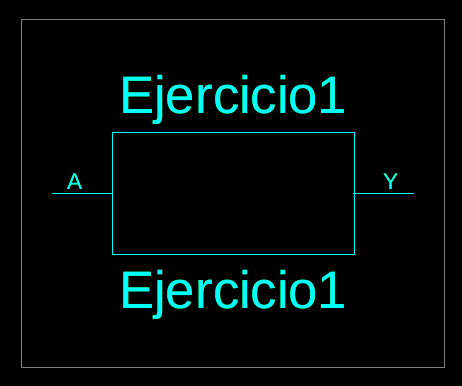
\includegraphics[width=0.5\textwidth]{rtl_ejercicio1.png}
	\caption{RTL generado para el ejercicio 1.}
	\label{fig:rtl_ejercicio1}
\end{figure}

\subsection{Verificación}

El funcionamiento esperado es que, cuando la llave conectada a la entrada $A$ se encuentre en estado lógico bajo, el LED permanezca apagado. Cuando la llave se encuentre en estado lógico alto, el LED conectado a la salida $Y$ se encienda.
\newpage
	
	
	
	\section{Ejercicio 2: Compuerta AND}
	
	\subsection{Consigna}
	
	Se desea diseñar una compuerta AND de dos entradas.
	
	\subsection{Entradas}
	
	\begin{itemize}
		\item $A$
		\item $B$
	\end{itemize}
	
	\subsection{Salida}
	
	\begin{itemize}
		\item $Y$
	\end{itemize}
	
	\subsection{Tabla de verdad}
	
	\begin{table}[h]
		\centering
		\begin{tabular}{|c|c|c|}
			\hline
			$A$ & $B$ & $Y$ \\ \hline
			0 & 0 & 0 \\ \hline
			0 & 1 & 0 \\ \hline
			1 & 0 & 0 \\ \hline
			1 & 1 & 1 \\ \hline
		\end{tabular}
		\caption{Tabla de verdad de la compuerta AND.}
		\label{tab:ej2_and}
	\end{table}
	
	\subsection{Análisis}
	
	A partir de la tabla de verdad se observa que la salida $Y$ toma el valor lógico alto únicamente cuando ambas entradas, $A$ y $B$, se encuentran en estado lógico alto.
	
	Por lo tanto, la función lógica del circuito es:
	
	\[
	Y = A \cdot B
	\]
	
	Esta expresión corresponde a una compuerta AND de dos entradas.
	
	\subsection{Código Verilog}
	
	\begin{verbatim}
		module ejercicio2 (
		input A,
		input B,
		output Y
		);
		
		assign Y = A & B;
		
		endmodule
	\end{verbatim}
	
	\subsection{Síntesis y RTL}
	
	Luego de realizar el código en Verilog, se sintetizó el diseño en Xilinx ISE. El RTL generado permite verificar que las entradas $A$ y $B$ ingresan a una compuerta AND, cuya salida corresponde a $Y$.
	
	\begin{figure}[h]
		\centering
		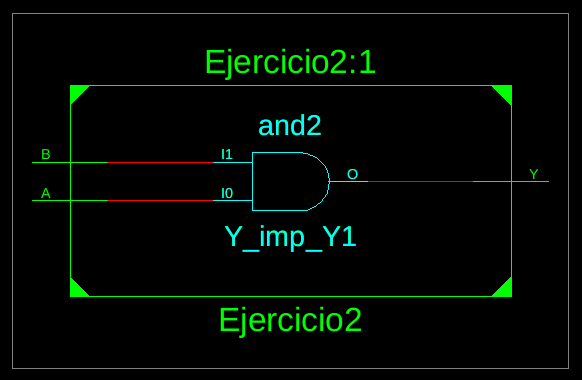
\includegraphics[width=0.75\textwidth]{rtl_ejercicio2.png}
		\caption{RTL generado para el ejercicio 2.}
		\label{fig:rtl_ejercicio2}
	\end{figure}
	
	\subsection{Verificación}
	
	El funcionamiento esperado es que el LED conectado a la salida $Y$ permanezca apagado cuando alguna de las entradas sea $0$. El LED se encenderá únicamente cuando las dos llaves conectadas a $A$ y $B$ estén en estado lógico $1$.
	\newpage
	
	
	

	\section{Ejercicio 3: Detector de mayoría}
	
	\subsection{Consigna}
	
	Se desea diseñar un circuito cuya salida sea igual a $1$ cuando al menos dos de sus entradas sean iguales a $1$.
	
	\subsection{Entradas}
	
	\begin{itemize}
		\item $A$
		\item $B$
		\item $C$
	\end{itemize}
	
	\subsection{Salida}
	
	\begin{itemize}
		\item $Y$
	\end{itemize}
	
	\subsection{Tabla de verdad}
	
	\begin{table}[h]
		\centering
		\begin{tabular}{|c|c|c|c|}
			\hline
			$A$ & $B$ & $C$ & $Y$ \\ \hline
			0 & 0 & 0 & 0 \\ \hline
			0 & 0 & 1 & 0 \\ \hline
			0 & 1 & 0 & 0 \\ \hline
			0 & 1 & 1 & 1 \\ \hline
			1 & 0 & 0 & 0 \\ \hline
			1 & 0 & 1 & 1 \\ \hline
			1 & 1 & 0 & 1 \\ \hline
			1 & 1 & 1 & 1 \\ \hline
		\end{tabular}
		\caption{Tabla de verdad del detector de mayoría.}
		\label{tab:ej3_mayoria}
	\end{table}
	
	\subsection{Análisis}
	
	A partir de la tabla de verdad se observa que la salida $Y$ toma el valor lógico alto cuando al menos dos entradas se encuentran en estado lógico $1$.
	
	Los casos en los que la salida vale $1$ son:
	
	\[
	ABC = 011,\ 101,\ 110,\ 111
	\]
	
	Por lo tanto, la función lógica puede expresarse como:
	
	\[
	Y = A \cdot B + A \cdot C + B \cdot C
	\]
	
	Esta expresión indica que la salida será $1$ si se cumple cualquiera de las siguientes condiciones:
	
	\begin{itemize}
		\item $A$ y $B$ valen $1$.
		\item $A$ y $C$ valen $1$.
		\item $B$ y $C$ valen $1$.
	\end{itemize}
	
	\subsection{Código Verilog}
	
	\begin{verbatim}
		module ejercicio3 (
		input A,
		input B,
		input C,
		output Y
		);
		
		assign Y = (A & B) | (A & C) | (B & C);
		
		endmodule
	\end{verbatim}
	
	\subsection{Síntesis y RTL}
	
	Luego de realizar el código en Verilog, se sintetizó el diseño en Xilinx ISE. El RTL generado permite verificar que la salida $Y$ se obtiene a partir de la combinación lógica de las entradas $A$, $B$ y $C$.
	
	\begin{figure}[H]
		\centering
		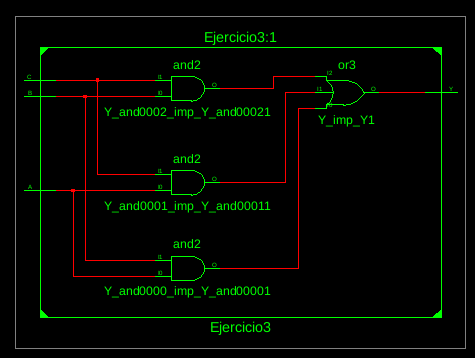
\includegraphics[width=0.75\textwidth]{rtl_ejercicio3.png}
		\caption{RTL generado para el ejercicio 3.}
		\label{fig:rtl_ejercicio3}
	\end{figure}
	
	\subsection{Verificación}
	
	El funcionamiento esperado es que la salida $Y$ permanezca en estado lógico bajo cuando ninguna entrada, o solamente una entrada, se encuentre en $1$. La salida se activa únicamente cuando dos o tres entradas se encuentran en estado lógico alto.
\newpage






\section{Ejercicio 4: Sistema de alarma}

\subsection{Consigna}

Se desea implementar un sistema de alarma para una vivienda. La alarma debe activarse cuando la puerta esté abierta o cuando la ventana esté abierta.

\subsection{Entradas}

\begin{itemize}
	\item $P$: puerta
	\item $V$: ventana
\end{itemize}

\subsection{Salida}

\begin{itemize}
	\item $A$: alarma
\end{itemize}

\subsection{Tabla de verdad}

\begin{table}[h]
	\centering
	\begin{tabular}{|c|c|c|}
		\hline
		$P$ & $V$ & $A$ \\ \hline
		0 & 0 & 0 \\ \hline
		0 & 1 & 1 \\ \hline
		1 & 0 & 1 \\ \hline
		1 & 1 & 1 \\ \hline
	\end{tabular}
	\caption{Tabla de verdad del sistema de alarma.}
	\label{tab:ej4_alarma}
\end{table}

\subsection{Análisis}

A partir de la tabla de verdad se observa que la salida $A$ se activa cuando al menos una de las entradas se encuentra en estado lógico alto.

Si la puerta está abierta, la alarma se activa. Si la ventana está abierta, la alarma también se activa. En caso de que ambas estén cerradas, la alarma permanece desactivada.

Por lo tanto, la función lógica del circuito es:

\[
A = P + V
\]

Esta expresión corresponde a una compuerta OR de dos entradas.
\newpage
\subsection{Código Verilog}

\begin{verbatim}
	module ejercicio4 (
	input P,
	input V,
	output A
	);
	
	assign A = P | V;
	
	endmodule
\end{verbatim}

\subsection{Síntesis y RTL}

Luego de realizar el código en Verilog, se sintetizó el diseño en Xilinx ISE. El RTL generado permite verificar que las entradas $P$ y $V$ ingresan a una compuerta OR, cuya salida corresponde a la alarma $A$.

\begin{figure}[h]
	\centering
	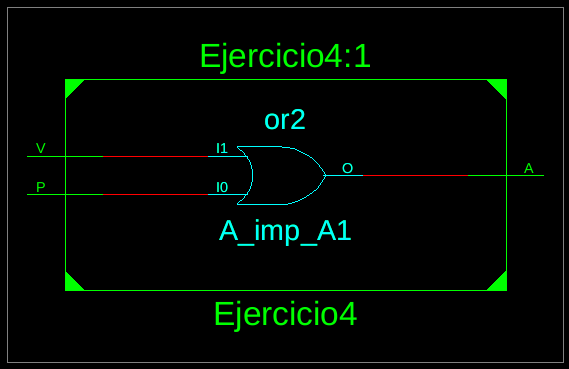
\includegraphics[width=0.75\textwidth]{rtl_ejercicio4.png}
	\caption{RTL generado para el ejercicio 4.}
	\label{fig:rtl_ejercicio4}
\end{figure}

\subsection{Verificación}

El funcionamiento esperado es que la alarma permanezca apagada cuando la puerta y la ventana estén cerradas. Si la puerta o la ventana se encuentran abiertas, la salida $A$ pasa a estado lógico alto, activando la alarma.
\newpage







\section{Ejercicio 5: Control de acceso}

\subsection{Consigna}

Se desea implementar un sistema de acceso. El acceso se habilita cuando existe una tarjeta válida y la contraseña es correcta.

\subsection{Entradas}

\begin{itemize}
	\item $T$: tarjeta válida
	\item $C$: contraseña correcta
\end{itemize}

\subsection{Salida}

\begin{itemize}
	\item $A$: acceso habilitado
\end{itemize}

\subsection{Tabla de verdad}

\begin{table}[h]
	\centering
	\begin{tabular}{|c|c|c|}
		\hline
		$T$ & $C$ & $A$ \\ \hline
		0 & 0 & 0 \\ \hline
		0 & 1 & 0 \\ \hline
		1 & 0 & 0 \\ \hline
		1 & 1 & 1 \\ \hline
	\end{tabular}
	\caption{Tabla de verdad del control de acceso.}
	\label{tab:ej5_acceso}
\end{table}

\subsection{Análisis}

A partir de la tabla de verdad se observa que la salida $A$ toma el valor lógico alto únicamente cuando ambas condiciones se cumplen al mismo tiempo: la tarjeta es válida y la contraseña es correcta.

Si una de las dos condiciones no se cumple, el acceso permanece deshabilitado.

Por lo tanto, la función lógica del circuito es:

\[
A = T \cdot C
\]

Esta expresión corresponde a una compuerta AND de dos entradas.
\newpage
\subsection{Código Verilog}

\begin{verbatim}
	module ejercicio5 (
	input T,
	input C,
	output A
	);
	
	assign A = T & C;
	
	endmodule
\end{verbatim}

\subsection{Síntesis y RTL}

Luego de realizar el código en Verilog, se sintetizó el diseño en Xilinx ISE. El RTL generado permite verificar que las entradas $T$ y $C$ ingresan a una compuerta AND, cuya salida corresponde a $A$.

\begin{figure}[h]
	\centering
	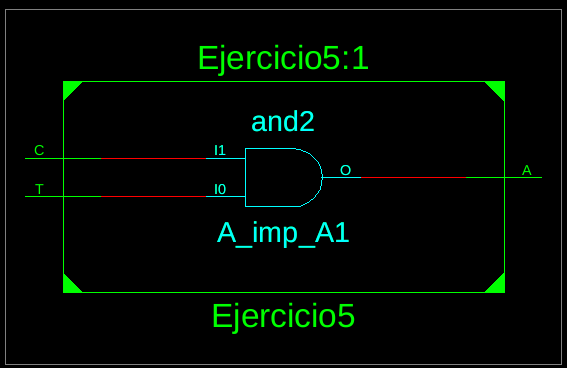
\includegraphics[width=0.75\textwidth]{rtl_ejercicio5.png}
	\caption{RTL generado para el ejercicio 5.}
	\label{fig:rtl_ejercicio5}
\end{figure}

\subsection{Verificación}

El funcionamiento esperado es que el acceso permanezca deshabilitado cuando la tarjeta no sea válida o cuando la contraseña sea incorrecta. La salida $A$ se activa únicamente cuando la tarjeta es válida y la contraseña es correcta.
\newpage











\section{Ejercicio 6: Control de acceso con supervisor}

\subsection{Consigna}

Se desea modificar el sistema de acceso del ejercicio anterior considerando que un supervisor puede habilitar el acceso independientemente de la tarjeta y la contraseña.

\subsection{Entradas}

\begin{itemize}
	\item $T$: tarjeta válida
	\item $C$: contraseña correcta
	\item $S$: supervisor
\end{itemize}

\subsection{Salida}

\begin{itemize}
	\item $A$: acceso habilitado
\end{itemize}

\subsection{Tabla de verdad}

\begin{table}[h]
	\centering
	\begin{tabular}{|c|c|c|c|}
		\hline
		$T$ & $C$ & $S$ & $A$ \\ \hline
		0 & 0 & 0 & 0 \\ \hline
		0 & 0 & 1 & 1 \\ \hline
		0 & 1 & 0 & 0 \\ \hline
		0 & 1 & 1 & 1 \\ \hline
		1 & 0 & 0 & 0 \\ \hline
		1 & 0 & 1 & 1 \\ \hline
		1 & 1 & 0 & 1 \\ \hline
		1 & 1 & 1 & 1 \\ \hline
	\end{tabular}
	\caption{Tabla de verdad del control de acceso con supervisor.}
	\label{tab:ej6_acceso_supervisor}
\end{table}

\subsection{Análisis}

A partir de la tabla de verdad se observa que el acceso se habilita cuando se cumplen simultáneamente las condiciones de tarjeta válida y contraseña correcta. Además, el acceso también se habilita si el supervisor se encuentra activo, independientemente del estado de las otras entradas.

Por lo tanto, la función lógica del circuito es:

\[
A = T \cdot C + S
\]

Esta expresión indica que la salida $A$ será igual a $1$ cuando $T$ y $C$ valgan $1$, o cuando $S$ valga $1$.

\subsection{Código Verilog}

\begin{verbatim}
	module ejercicio6 (
	input T,
	input C,
	input S,
	output A
	);
	
	assign A = (T & C) | S;
	
	endmodule
\end{verbatim}

\subsection{Síntesis y RTL}

Luego de realizar el código en Verilog, se sintetizó el diseño en Xilinx ISE. El RTL generado permite verificar que las entradas $T$ y $C$ ingresan a una compuerta AND, y el resultado se combina mediante una compuerta OR con la entrada $S$.

\begin{figure}[h]
	\centering
	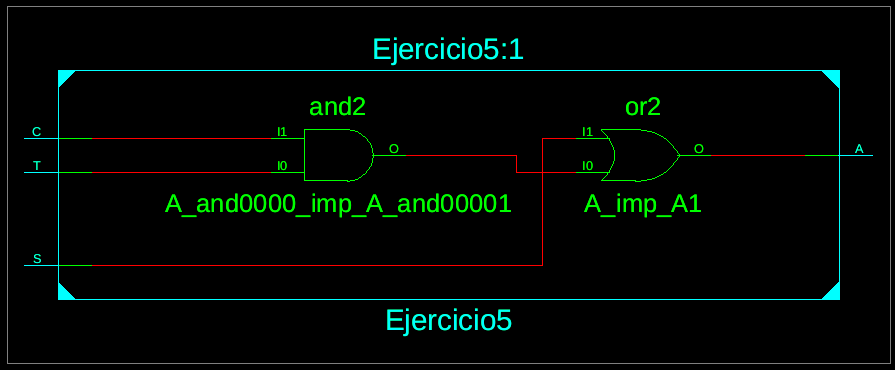
\includegraphics[width=0.75\textwidth]{rtl_ejercicio6.png}
	\caption{RTL generado para el ejercicio 6.}
	\label{fig:rtl_ejercicio6}
\end{figure}

\subsection{Verificación}

El funcionamiento esperado es que el acceso permanezca deshabilitado cuando no se cumplan las condiciones de tarjeta válida y contraseña correcta, y cuando el supervisor no esté activo. La salida $A$ se activa si la tarjeta es válida y la contraseña es correcta, o si el supervisor habilita el acceso.
\newpage







\section{Ejercicio 7: Multiplexor 2:1}

\subsection{Consigna}

Se desea diseñar un multiplexor $2:1$. Este circuito permite seleccionar una de dos entradas de datos y enviarla a una única salida, dependiendo del valor de una señal de selección.

\subsection{Entradas}

\begin{itemize}
	\item $I0$: entrada de datos 0
	\item $I1$: entrada de datos 1
	\item $SEL$: señal de selección
\end{itemize}

\subsection{Salida}

\begin{itemize}
	\item $Y$: salida del multiplexor
\end{itemize}

\subsection{Funcionamiento}

El funcionamiento del multiplexor $2:1$ está determinado por la entrada de selección $SEL$.

\begin{table}[h]
	\centering
	\begin{tabular}{|c|c|}
		\hline
		$SEL$ & $Y$ \\ \hline
		0 & $I0$ \\ \hline
		1 & $I1$ \\ \hline
	\end{tabular}
	\caption{Funcionamiento del multiplexor $2:1$.}
	\label{tab:ej7_funcionamiento}
\end{table}

\subsection{Tabla de verdad completa}

\begin{table}[h]
	\centering
	\begin{tabular}{|c|c|c|c|}
		\hline
		$SEL$ & $I0$ & $I1$ & $Y$ \\ \hline
		0 & 0 & 0 & 0 \\ \hline
		0 & 0 & 1 & 0 \\ \hline
		0 & 1 & 0 & 1 \\ \hline
		0 & 1 & 1 & 1 \\ \hline
		1 & 0 & 0 & 0 \\ \hline
		1 & 0 & 1 & 1 \\ \hline
		1 & 1 & 0 & 0 \\ \hline
		1 & 1 & 1 & 1 \\ \hline
	\end{tabular}
	\caption{Tabla de verdad completa del multiplexor $2:1$.}
	\label{tab:ej7_mux21}
\end{table}

\subsection{Análisis}

A partir de la tabla de funcionamiento se observa que la salida $Y$ depende de la señal de selección $SEL$.

Cuando $SEL = 0$, la salida debe tomar el valor de la entrada $I0$. Para representar esta condición se utiliza el término:

\[
\overline{SEL} \cdot I0
\]

Cuando $SEL = 1$, la salida debe tomar el valor de la entrada $I1$. Para representar esta condición se utiliza el término:

\[
SEL \cdot I1
\]

Por lo tanto, la función lógica del multiplexor $2:1$ queda expresada como:

\[
Y = \overline{SEL} \cdot I0 + SEL \cdot I1
\]

\subsection{Código Verilog}

\begin{verbatim}
	module ejercicio7 (
	input I0,
	input I1,
	input SEL,
	output Y
	);
	
	assign Y = (~SEL & I0) | (SEL & I1);
	
	endmodule
\end{verbatim}


También puede implementarse de forma equivalente utilizando el operador condicional ternario: \begin{verbatim} module ejercicio7 ( 
	input I0, 
	input I1, 
	input SEL, 
	output Y 
	); 
	
	assign Y = SEL ? I1 : I0; 
	
	endmodule 
	\end{verbatim} 
	En esta segunda implementación, la instrucción: 
	\begin{verbatim} 
	assign Y = SEL ? I1 : I0; 
	\end{verbatim} 
		indica que si $SEL = 1$, la salida $Y$ toma el valor de $I1$. En cambio, si $SEL = 0$, la salida $Y$ toma el valor de $I0$. Por lo tanto, ambas formas describen el mismo funcionamiento del multiplexor $2:1$.



\subsection{Síntesis y RTL}

Luego de realizar el código en Verilog, se sintetizó el diseño en Xilinx ISE. El RTL generado permite verificar que la salida $Y$ se obtiene seleccionando una de las dos entradas, $I0$ o $I1$, según el valor de la señal $SEL$.

\begin{figure}[h]
	\centering
	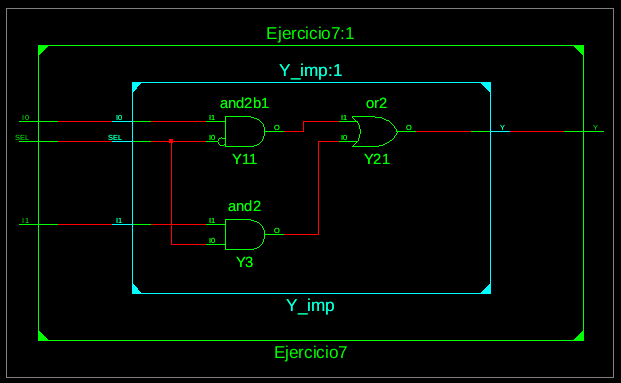
\includegraphics[width=0.75\textwidth]{rtl_ejercicio7.png}
	\caption{RTL generado para el ejercicio 7.}
	\label{fig:rtl_ejercicio7}
\end{figure}

\subsection{Verificación}

El funcionamiento esperado es que, cuando la señal $SEL$ se encuentre en estado lógico bajo, la salida $Y$ copie el valor de la entrada $I0$. Cuando $SEL$ se encuentre en estado lógico alto, la salida $Y$ copie el valor de la entrada $I1$.
\newpage






\section{Ejercicio 8: Multiplexor 4:1}

\subsection{Consigna}

Se desea diseñar un multiplexor $4:1$ utilizando la ecuación lógica correspondiente. Este circuito permite seleccionar una de cuatro entradas de datos y enviarla a una única salida, dependiendo del valor de las señales de selección.

\subsection{Entradas}

\begin{itemize}
	\item $I0$: entrada de datos 0
	\item $I1$: entrada de datos 1
	\item $I2$: entrada de datos 2
	\item $I3$: entrada de datos 3
	\item $S1$: bit más significativo de selección
	\item $S0$: bit menos significativo de selección
\end{itemize}

\subsection{Salida}

\begin{itemize}
	\item $Y$: salida del multiplexor
\end{itemize}

\subsection{Funcionamiento}

El funcionamiento del multiplexor $4:1$ depende de las señales de selección $S1$ y $S0$.

\begin{table}[h]
	\centering
	\begin{tabular}{|c|c|c|}
		\hline
		$S1$ & $S0$ & $Y$ \\ \hline
		0 & 0 & $I0$ \\ \hline
		0 & 1 & $I1$ \\ \hline
		1 & 0 & $I2$ \\ \hline
		1 & 1 & $I3$ \\ \hline
	\end{tabular}
	\caption{Funcionamiento del multiplexor $4:1$.}
	\label{tab:ej8_funcionamiento}
\end{table}

\subsection{Tabla de verdad}

\begin{table}[H]
	\centering
	\begin{tabular}{|c|c|c|c|c|c|c|}
		\hline
		$S1$ & $S0$ & $I0$ & $I1$ & $I2$ & $I3$ & $Y$ \\ \hline
		0 & 0 & 0 & X & X & X & 0 \\ \hline
		0 & 0 & 1 & X & X & X & 1 \\ \hline
		0 & 1 & X & 0 & X & X & 0 \\ \hline
		0 & 1 & X & 1 & X & X & 1 \\ \hline
		1 & 0 & X & X & 0 & X & 0 \\ \hline
		1 & 0 & X & X & 1 & X & 1 \\ \hline
		1 & 1 & X & X & X & 0 & 0 \\ \hline
		1 & 1 & X & X & X & 1 & 1 \\ \hline
	\end{tabular}
	\caption{Tabla de verdad resumida del multiplexor $4:1$.}
	\label{tab:ej8_mux41}
\end{table}

\subsection{Análisis}

A partir de la tabla de funcionamiento se observa que la salida $Y$ depende de las señales de selección $S1$ y $S0$.

Cuando $S1=0$ y $S0=0$, la salida toma el valor de $I0$:

\[
\overline{S1} \cdot \overline{S0} \cdot I0
\]

Cuando $S1=0$ y $S0=1$, la salida toma el valor de $I1$:

\[
\overline{S1} \cdot S0 \cdot I1
\]

Cuando $S1=1$ y $S0=0$, la salida toma el valor de $I2$:

\[
S1 \cdot \overline{S0} \cdot I2
\]

Cuando $S1=1$ y $S0=1$, la salida toma el valor de $I3$:

\[
S1 \cdot S0 \cdot I3
\]

Por lo tanto, la función lógica del multiplexor $4:1$ queda expresada como:

\[
Y = \overline{S1} \cdot \overline{S0} \cdot I0 + 
\overline{S1} \cdot S0 \cdot I1 +
S1 \cdot \overline{S0} \cdot I2 +
S1 \cdot S0 \cdot I3
\]

\subsection{Código Verilog}

El multiplexor $4:1$ se implementó en Verilog utilizando la ecuación lógica obtenida anteriormente:

\begin{verbatim}
	module ejercicio8 (
	input I0,
	input I1,
	input I2,
	input I3,
	input S1,
	input S0,
	output Y
	);
	
	assign Y = (~S1 & ~S0 & I0) |
	(~S1 &  S0 & I1) |
	( S1 & ~S0 & I2) |
	( S1 &  S0 & I3);
	
	endmodule
\end{verbatim}

También puede implementarse de forma equivalente utilizando el operador condicional ternario:

\begin{verbatim}
	module ejercicio8 (
	input I0,
	input I1,
	input I2,
	input I3,
	input S1,
	input S0,
	output Y
	);
	
	assign Y = ({S1,S0} == 2'b00) ? I0 :
	({S1,S0} == 2'b01) ? I1 :
	({S1,S0} == 2'b10) ? I2 :
	I3;
	
	endmodule
\end{verbatim}

\subsection{Síntesis y RTL}

Luego de realizar el código en Verilog, se sintetizó el diseño en Xilinx ISE. El RTL generado permite verificar que las señales de selección $S1$ y $S0$ determinan cuál de las cuatro entradas se conecta a la salida $Y$.

\begin{figure}[H]
	\centering
	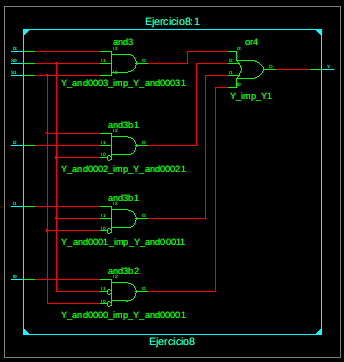
\includegraphics[width=0.8\textwidth]{rtl_ejercicio8.png}
	\caption{RTL generado para el ejercicio 8.}
	\label{fig:rtl_ejercicio8}
\end{figure}

\subsection{Verificación}

El funcionamiento esperado es que la salida $Y$ copie el valor de una de las cuatro entradas según el valor de las señales de selección. Si $S1S0 = 00$, la salida toma el valor de $I0$; si $S1S0 = 01$, toma el valor de $I1$; si $S1S0 = 10$, toma el valor de $I2$; y si $S1S0 = 11$, toma el valor de $I3$.



	
\end{document}